
\chapter{Débuter avec HTML/CSS}
Ce court tutoriel est destiné à  ceux qui commencent à  utiliser CSS et n'ont jamais écrit de feuille de style CSS.

Il n'explique pas CSS en profondeur. Il explique comment créer un fichier HTML, un fichier CSS et comment les faire fonctionner ensemble. Après cela, vous pourrez lire d'autres tutoriels afin d'ajouter plus de caractéristiques à  vos fichiers HTML et CSS. Ou bien vous pouvez utiliser un éditeur HTML ou CSS afin de mettre en place des sites complexes.

A la fin de ce tutoriel, vous aurez fait un fichier HTML qui ressemble à cela (voir figure \ref{fig:screen1}). 

\begin{figure}[h]
	\begin{center}
		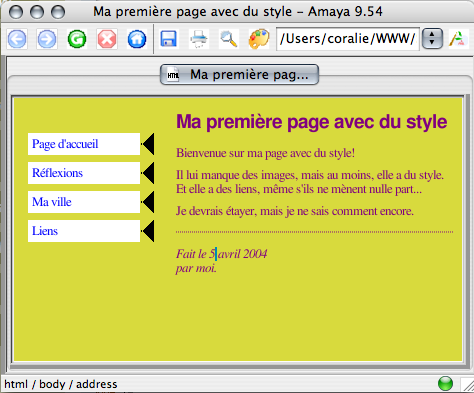
\includegraphics{voronin/img/capture5.png}	
		\caption{Page HTML résultante, couleurs et disposition effectuées avec CSS.}
		\label{fig:screen1}
	\end{center}
\end{figure}
Notez que je ne prétends pas que c'est joli :)
\alerte{3}{l}
Voici un exemple de section \emph{optionnelle}. Elles contiennent des explications supplémentaires du langage HTML et TML et du code CSS des exemples. L'icône "alerte!" qui les précède indique que la section contient des informations plus avancées que le reste.
\normalsize
\section{Le langage HTML}
Pour ce tutoriel, je vous recommande d'utiliser des outils simples comme Blocnote (Windows), TextEdit (Mac) ou KEdit (KDE). Une fois que vous aurez intégré ces principes, vous pourrez facilement utiliser des outils plus avancés, ou des logiciels commerciaux tels que Style Master, Dreamweaver ou GoLive. Cependant pour votre première feuille de style CSS, il vaut mieux que vous ne soyez pas distrait par de nombreuses caractéristiques avancées.

N'utilisez pas un logiciel de traitement de texte, tels que Microsoft Word ou OpenOffice, car ils produisent des fichiers qu'un navigateur Web ne sait pas lire. Pour HTML et CSS, nous voulons de simples fichiers texte.

\textbf{L'étape 1} est d'ouvrir votre éditeur de texte (Notepad, TextEdit, KEdit, etc., quel que soit votre éditeur favori), de commencer avec une fenêtre vide et de taper ceci:
\begin{lstlisting}[language=html]
	<!DOCTYPE html PUBLIC "-//W3C//DTD HTML 4.01//EN">
	<html>
	<head>
	<title>Ma premiere page avec du style</title>
	</head>
	
	<body>
	
	<!-- Menu de navigation du site -->
	<ul class="navbar">
	<li><a href="index.html">Home page</a>
	<li><a href="reflexions.html">Reflexions</a>
	<li><a href="ville.html">Ma ville</a>
	<li><a href="liens.html">Liens</a>
	</ul>
	
	<!-- Contenu principal -->
	<h1>Ma premiere page avec du style</h1>
	
	<p>Bienvenue sur ma page avec du style! 
	
	<p>Il lui manque des images, mais au moins, elle a du style. Et elle a des liens, meme s'ils ne menent nulle part...
	&hellip;
	
	<p>Je devrais etayer, mais je ne sais comment encore.
	
	<!-- Signer et dater la page, c'est une question de politesse! -->
	<address>Fait le 5 avril 2004<br>
	par moi.</address>
	</body>
	</html>
\end{lstlisting}
En fait, vous n'avez pas à le taper: vous pouvez le copier et coller depuis cette page Web dans votre éditeur.

(Si vous utilisez TextEdit sur Mac, n'oubliez pas de dire à TextEdit qu'il s'agit de texte simple; pour ceci, allez au menu Format et sélectionnez "Convertir au format Texte".) 
\alerte{13}{l}
 La première ligne du fichier HTML ci-dessus dit au navigateur de quel type d'HTML il s'agit (DOCTYPE signifie DOCument TYPE). Dans ce cas, il s'agit de la version 4.01 d'HTML.
 
 Les mots à l'intérieur de < et > sont nommés balises et comme vous pouvez le voir, le document est contenu à l'intérieur des balises <html> et </html>. Entre <head> et </head> se trouve la place pour des informations variées qui ne sont pas affichées à l'écran. A ce stade, il contient le titre du document, mais plus tard, nous y ajouterons la feuille de style CSS.
 
 Le <body> est l'emplacement du texte à proprement parler de notre document. En principe, tout ce qui s'y trouve sera affiché, à l'exception du texte contenu entre entre <!-- et -->, qui sert de commentaire pour nous-même. Le navigateur ignorera ce texte.
 
 Parmi les balises de l'exemple, <ul> introduit une "Liste non ordonnée", c'est à dire une liste dans laquelle les éléments ne sont pas numérotés. La balise <li> est le début d'un "élément de liste ". Le <p> est un "paragraphe". Et le <a> est une "ancre", ce qui crée un hyperlien(voir figure \ref{fig:screen2}). 

\begin{figure}[t]
	\begin{center}
		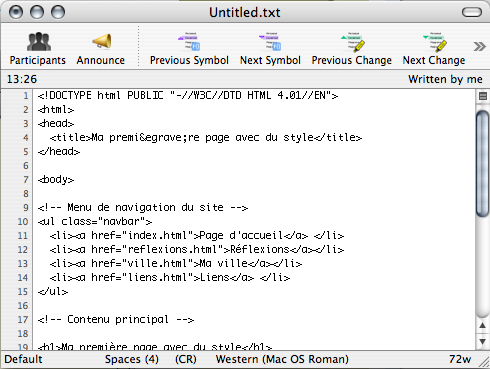
\includegraphics{voronin/img/capture.png}
		\caption{L'éditeur Subethaedit affichant le code source HTML.}
		\label{fig:screen2}		
	\end{center}
\end{figure}
\alerte{11}{l}
Si vous désirez connaître la signification du contenu d'un <…>, je vous recommande de commencer avec Getting started with HTML. Mais permettez-moi de vous livrer quelques mots sur la structure de la page HTML en exemple.
\begin{itemize}
	\item Le "ul" est une liste avec un hyperlien par élément. Cela nous servira de "menu de navigation de site," nous créerons des liens vers les autres pages de notre (hypothétique) site Web. Nous présumons que toutes les pages sur notre site ont un menu similaire.
	\item Les éléments "h1" et "p" forment le contenu unique de cette page, et la signature en bas ("address") sera similaire sur toutes les pages du site. 
\end{itemize}
Notez que je n'ai pas fermé les éléments "li" et "p". En langage HTML (mais pas en XHTML), il est permis d'omettre les balises </li> et </p>, ce que j'ai fait là, afin de rendre le texte un peu plus facile à lire. Mais vous pouvez les ajouter, si vous préférez. 
\normalsize

Admettons qu'il s'agira d'une page d'un site Web contenant plusieurs pages similaires. Comme dans beaucoup de pages Web actuelles, celle-ci a un menu avec des liens vers d'autres pages de notre site hypothétique, un contenu unique ainsi qu'une signature.

Sélectionnez maintenant "Sauver-sous…" depuis votre menu Fichier, naviguez vers le répertoire/dossier où vous voulez sauver votre fichier (le Bureau est tout à fait convenable) et sauvez le fichier sous le nom "mapage.html". Ne fermez pas l'éditeur car nous en aurons encore besoin.

(Si vous utilisez TextEdit sur Mac OS X avant version 10.4, vous voyez une option pour ne pas ajouter l'extension .txt. Sélectionnez cette option, parce que "mapage.html" a déjà une extension. Les versions plus récentes de TextEdit remarquent l'extension .html automatiquement.)

Ensuite, ouvrez le fichier dans un navigateur. Vous pouvez faire cela comme suit: cherchez le fichier avec votre explorateur de fichiers (Explorateur Windows, Finder ou Konqueror) et cliquez ou double-cliquez sur le fichier "mapage.html". Il devrait s'ouvrir dans votre navigateur Web par défaut. (Si ce n'est pas le cas, ouvrez votre navigateur et cliquez-déplacez le fichier dans le navigateur.)

Comme vous pouvez le voir, la page est assez ennuyeuse… 
\section{Ajouter de la couleur}
Vous voyez probablement du texte noir sur un fond blanc, mais cela dépend de la façon dont le navigateur est configuré. Une manière simple de rendre la page plus stylée et d'y ajouter des couleurs. (Laissez votre navigateur ouvert, nous l'utiliserons à nouveau plus tard.)

Nous allons commencer avec une feuille de style intégrée dans le fichier HTML. Par la suite, nous nous mettrons le HTML et le CSS dans des fichiers séparés. Séparer les fichiers est une bonne chose car cela vous permet facilement d'utiliser la même feuille de style sur plusieurs fichiers HTML: il vous suffit d'écrire votre feuille de style une fois. Mais pour cette cette étape, nous écrirons tout dans notre seul fichier.

Nous devons ajouter un élément <style> au fichier HTML. La feuille de style sera dans cet élément. Retournez à la fenêtre de votre éditeur et ajoutez les cinq lignes suivantes dans la partie head de votre fichier HTML. Les lignes à ajouter sont affichées en rouge. 
\begin{lstlisting}[language=html]
	<!DOCTYPE html PUBLIC "-//W3C//DTD HTML 4.01//EN">
	<html>
	<head>
	<title>Ma premiere page avec du style</title>
	<style type="text/css">
	body {
		color: purple;
		background-color: #d8da3d }
	</style>
	</head>
	
	<body>
	[etc.]
\end{lstlisting}
La première ligne indique qu'il s'agit d'une feuille de style et qu'elle est écrite en CSS ("text/css"). La seconde ligne indique que nous ajoutons du style à l'élément "body". La troisième ligne indique que la couleur du texte sera le violet, et la ligne suivante que le fond aura comme couleur une sorte de jaune verdâtre. 
\alerte{12}{l}
Les feuilles de style en CSS sont constituées de règles. Chacune des règles est en trois partie:
\begin{enumerate}
	\item Le sélecteur (dans l'exemple: "body"), qui indique au navigateur quelle partie du document est affectée par la règle;
	\item La propriété (dans l'exemple, 'color' et 'background-color' sont des propriétés), qui spécifie quel aspect de l'affichage est paramétré
	\item Et la valeur ('purple' et '\#d8da3d'), qui indique la valeur de la propriété de style. 
\end{enumerate}
L'exemple montre que les règles peuvent être combinées. Nous avons paramétré deux propriétés, donc nous aurions pu en faire deux règles séparées:

\begin{lstlisting}[language=html]
	body { color: purple }
	body { background-color: #d8da3d }
\end{lstlisting}

Mais puisque les deux règles affectent le corps ("body"), nous avons indiqué "body" une seule fois et mis les propriétés et valeurs ensemble. Pour en savoir plus sur les sélecteurs, se reporter au chapitre 2 de Lie \& Bos. 
\normalsize

Le fond de l'élément "body" sera également le fond de tout le document. Nous n'avons pas donné aux autres éléments (p, li, address…) de valeur explicite sur le fond, donc par défaut, ils n'en auront pas (ou plutôt: ils seront transparents). La propriété 'color' détermine la couleur du texte de l'élément "body", mais tous les autres éléments dans le corps hériteront de cette couleur, à moins qu'une autre soit spécifiée (Nous ajouterons d'autres couleurs plus plus tard.)

Sauvez maintenant ce fichier (utilisez "Sauver" depuis le menu Fichier) et retournez à la fenêtre de votre navigateur. Si vous pressez l'icône "Recharger", l'affichage devrait changer de la page "ennuyeuse" à une page colorée (mais certes toujours ennuyeuse) A part la liste de liens en haut, le texte devrait maintenant être violet sur un fond jaune verdâtre (voir figure \ref{fig:screen3}). 
\begin{figure}[t]
	\begin{center}
		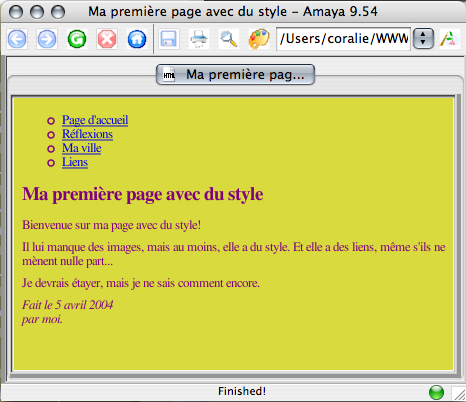
\includegraphics{voronin/img/capture2.png}	
		\caption{Voici comment un navigateur affiche la page maintenant que des couleurs ont été ajoutées. }
		\label{fig:screen3}
	\end{center}
\end{figure}
\alerte{6}{l}
En CSS, les couleurs peuvent être spécifiées de plusieurs manières. Cet exemple en montre deux: par nom ("purple") et par code hexadécimal ("\#d8da3d"). Il y a à peu prés 140 noms de couleurs. Les codes hexadécimaux permettent plus de 16 millions de couleurs. Adding a touch of style fournit plus d'explications à propos de ces codes. 
\normalsize
\section{Ajouter des fontes}
Une autre chose simple à faire est de distinguer les fontes des différents éléments de la page. Choisissons la fonte "Georgia", sauf pour le texte des titres de type h1 pour lesquels nous choisirons la fonte "Helvetica."

Sur le Web, vous ne pouvez jamais être sûr des fontes qu'auront vos lecteurs sur leurs ordinateurs, donc nous ajouterons des alternatives: si Georgia n'est pas disponible, Times New Roman ou Times iront très bien, et si ces deux-la sont également indisponibles, le navigateur pourra utiliser une autre fonte dans la famille serifs. Si Helvetica est absente, Geneva, Arial et SunSans-Regular sont assez similaire en forme, et si aucune de celles-ci ne fonctionne, le navigateur pourra choisir une autre fonte sans serif.

Dans votre éditeur de texte, ajoutez les lignes suivantes : 
\begin{lstlisting}[language=html]
	<!DOCTYPE html PUBLIC "-//W3C//DTD HTML 4.01//EN">
	<html>
	<head>
	<title>Ma premiere page avec du style</title>
	<style type="text/css">
	body {
		font-family: Georgia, "Times New Roman",
		Times, serif;
		color: purple;
		background-color: #d8da3d }
	h1 {
		font-family: Helvetica, Geneva, Arial,
		SunSans-Regular, sans-serif }
	</style>
	</head>
	
	<body>
	[etc.]
\end{lstlisting}
Si vous sauvez à nouveau et pressez "Recharger" dans le navigateur, vous devriez voir des fontes différentes pour le titre et le reste du texte (voir figure \ref{fig:screen4}).
\begin{figure}[t]
	\begin{center}
		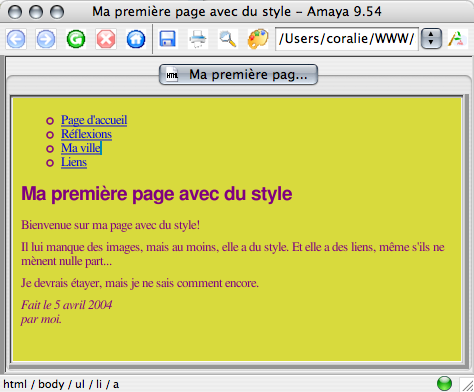
\includegraphics{voronin/img/capture3.png}	
		\caption{Maintenant le texte principal a une fonte différente de celle du titre.  }
		\label{fig:screen4}
	\end{center}
\end{figure} 
\section{La barre de navigation}
La liste en haut de la page HTML est sensée devenir un menu de navigation. Beaucoup de sites Web ont une sorte de menu en haut ou sur le côté de la page, et notre page devrait en avoir un aussi. Nous le mettrons du côté gauche, parce que c'est un peu plus intéressant qu'en haut…

Le menu est déjà dans la page HTML. Il s'agit de la liste <ul> en haut. Les liens à l'intérieur ne fonctionnent pas, puisque notre notre "site Web" consiste en une seule page, jusqu'à présent, donc ceci importe peu. Dans un site Web réel, il ne devrait pas y avoir de lien cassé, évidemment.

Nous devons donc déplacer la liste à gauche, et le reste du texte un petit peu à droite, pour faire de la place pour notre menu. Les propriétés CSS que nous utiliserons pour cela sont 'padding-left' (pour déplacer le texte du corps) et 'position', 'left' et 'top' (pour déplacer le menu).

Il y a d'autres manières de le faire. Si vous recherchez "column" ou "layout" dans la page Learning CSS, vous trouverez plusieurs modèles prêt à l'emploi. Mais cette manière convient à nos besoins.

Dans la fenêtre d'édition, ajoutez les lignes suivantes au fichier HTML : 
\begin{lstlisting}[language=html]
	<!DOCTYPE html PUBLIC "-//W3C//DTD HTML 4.01//EN">
	<html>
	<head>
	<title>Ma premiere page avec du style</title>
	<style type="text/css">
	body {
		padding-left: 11em;
		font-family: Georgia, "Times New Roman",
		Times, serif;
		color: purple;
		background-color: #d8da3d }
	ul.navbar {
		position: absolute;
		top: 2em;
		left: 1em;
		width: 9em }
	h1 {
		font-family: Helvetica, Geneva, Arial,
		SunSans-Regular, sans-serif }
	</style>
	</head>
	
	<body>
	[etc.]
\end{lstlisting}

Si vous sauvez encore et rechargez la page dans votre navigateur, vous devriez maintenant avoir la liste de liens à gauche du texte principal. C'est déjà bien plus intéressant, n'est-ce pas? (voir figure \ref{fig:screen5})
\begin{figure}[t]
	\begin{center}
		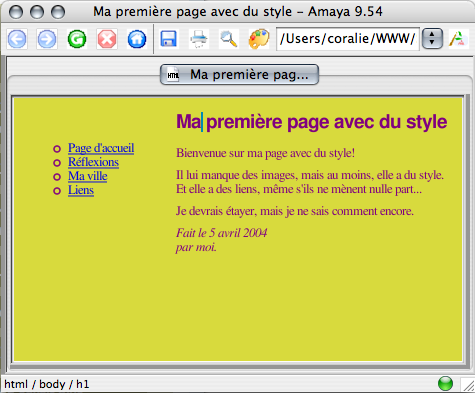
\includegraphics{voronin/img/capture4.png}	
		\caption{Le texte principal a été déplacé à droite et la liste de liens est maintenant à sa gauche au lieu d'être au-dessus. }
		\label{fig:screen5}
	\end{center}
\end{figure}
\alerte{12}{l}
'position: absolute' précise que l'élément ul est positionné de façon indépendante de tout texte qui vient avant ou après dans le document, et 'left' et 'top' indiquent quelle est cette position. Dans ce cas, 2em depuis le haut et 1em depuis le côté gauche de cette fenêtre.

'2em' signifie 2 fois la taille de la fonte courante. C'est à dire que si le menu est affiché avec une fonte de 12 points, '2em' font 24 points. L'unité 'em' est très utile en CSS puisqu'elle peut s'adapter automatiquement à la fonte que le lecteur utilise. La plupart des navigateurs ont un menu pour agrandir et réduire la taille de fonte: vous pouvez l'essayer et voir comment la taille du menu augmente dès que la fonte grossit, ce qui n'aurait pas été le cas si nous avions utilisé une taille en pixels à la place. 
\normalsize
\section{Stylisez vos liens}
Le menu de navigation ressemble toujours à une liste au lieu d'un menu. Ajoutons un peu de style. Nous allons supprimer les points de la liste et déplacer les éléments à gauche, à l'endroit où étaient les points. Nous allons aussi donner à chaque élément son propre fond blanc ainsi qu'un carré noir. (Pourquoi? Aucune raison en particulier, si ce n'est que l'on peut le faire.)

Nous n'avons pas déterminé quelle couleur auront les liens, alors nous ajouterons cela également: bleu pour les liens que l'utilisateur n'a pas encore vu et violet pour les liens déjà visités : 
\begin{lstlisting}[language=html]
	<!DOCTYPE html PUBLIC "-//W3C//DTD HTML 4.01//EN">
	<html>
	<head>
	<title>Ma premiere page avec du style</title>
	<style type="text/css">
	body {
	padding-left: 11em;
	font-family: Georgia, "Times New Roman",
	Times, serif;
	color: purple;
	background-color: #d8da3d }
	ul.navbar {
	list-style-type: none;
	padding: 0;
	margin: 0;
	position: absolute;
	top: 2em;
	left: 1em;
	width: 9em }
	h1 {
	font-family: Helvetica, Geneva, Arial,
	SunSans-Regular, sans-serif }
	ul.navbar li {
	background: white;
	margin: 0.5em 0;
	padding: 0.3em;
	border-right: 1em solid black }
	ul.navbar a {
	text-decoration: none }
	a:link {
	color: blue }
	a:visited {
	color: purple }
	</style>
	</head>
	
	<body>
	[etc.]
\end{lstlisting}
\alerte{12}{l}
Traditionellement, les navigateurs montrent les hyperliens soulignés et en couleurs. Habituellement, les couleurs sont similaires à celles que nous avons spécifiées ici: bleu pour les liens vers des pages qui n'ont pas encore été visitées (ou visitées il y a longtemps), violet pour les pages qui ont été déjà visitées.

En HTML, les hyperliens sont créés avec l'élément <a>, donc pour préciser la couleur, nous devons ajouter une règle de style pour "a". Afin de différencier les liens visités et les liens non visités, CSS propose deux "pseudo-classes" (:link et :visited). Elles sont appelées "pseudo-classes" pour les distinguer des classes attributs, qui apparaissent directement dans le HTML, c'est à dire, la classe class="navbar" dans notre exemple. 
\normalsize
\section{Ligne horizontale}
L'ajout final à notre feuille de style est une ligne horizontale pour séparer le texte de la signature en bas. Nous utiliserons 'border-top' afin d'ajouter une ligne en pointillé au-dessus de l'élément <address> : 
\begin{lstlisting}[language=html]
	<!DOCTYPE html PUBLIC "-//W3C//DTD HTML 4.01//EN">
	<html>
	<head>
	<title>Ma premiere page avec du style</title>
	<style type="text/css">
	body {
	padding-left: 11em;
	font-family: Georgia, "Times New Roman",
	Times, serif;
	color: purple;
	background-color: #d8da3d }
	ul.navbar {
	list-style-type: none;
	padding: 0;
	margin: 0;
	position: absolute;
	top: 2em;
	left: 1em;
	width: 9em }
	h1 {
	font-family: Helvetica, Geneva, Arial,
	SunSans-Regular, sans-serif }
	ul.navbar li {
	background: white;
	margin: 0.5em 0;
	padding: 0.3em;
	border-right: 1em solid black }
	ul.navbar a {
	text-decoration: none }
	a:link {
	color: blue }
	a:visited {
	color: purple }
	address {
	margin-top: 1em;
	padding-top: 1em;
	border-top: thin dotted }
	</style>
	</head>
	
	<body>
	[etc.]
\end{lstlisting}
Notre style est désormais terminé. Maintenant, penchons-nous sur comment faire de notre feuille de style un fichier à part, de sorte que d'autres pages peuvent partager le même style. 
\section{Mettre la feuille de style dans un fichier à part}
Nous disponsons d'un fichier HTML avec une feuille de style intégrée. Mais si notre site se développe, nous voulons probablement que plusieurs pages partagent le même style. Il existe une meilleure méthode que de copier la feuille de style dans chaque page: si nous mettons la feuille de style dans un fichier à part, toutes les pages peuvent pointer sur celui-ci.

Pour créer un fichier de feuille de style, nous devons créer un autre fichier texte vide. Vous pouvez sélectionner "Nouveau" depuis le menu Fichier de votre éditeur pour obtenir une fenêtre vide. (Si vous utilisez TextEdit, n'oubliez pas de forcer le texte simple à nouveau, en utilisant le menu Format.)

Ensuite, coupez et collez le contenu de l'élément <style> depuis le fichier HTML vers la nouvelle fenêtre. Ne copiez pas les éléments <style> et </style>. Ils appartiennent au langage HTML, pas à CSS. Dans la nouvelle fenêtre d'édition, vous devriez maintenant avoir la feuille de style complète: 
\begin{lstlisting}[language=html]
	body {
	padding-left: 11em;
	font-family: Georgia, "Times New Roman",
	Times, serif;
	color: purple;
	background-color: #d8da3d }
	ul.navbar {
	list-style-type: none;
	padding: 0;
	margin: 0;
	position: absolute;
	top: 2em;
	left: 1em;
	width: 9em }
	h1 {
	font-family: Helvetica, Geneva, Arial,
	SunSans-Regular, sans-serif }
	ul.navbar li {
	background: white;
	margin: 0.5em 0;
	padding: 0.3em;
	border-right: 1em solid black }
	ul.navbar a {
	text-decoration: none }
	a:link {
	color: blue }
	a:visited {
	color: purple }
	address {
	margin-top: 1em;
	padding-top: 1em;
	border-top: thin dotted }
\end{lstlisting}
Choisissez "Sauver-sous…" depuis le menu Fichier, assurez-vous que vous êtes dans le même répertoire/dossier où vous avez enregistré le fichier mapage.html, et sauvez la feuille de style sous le nom "monstyle.css".

Revenez maintenant à la fenêtre contenant le code HTML. Supprimez tout depuis la balise <style> jusqu'après la balise </style> et remplacez par l'élément <link> comme suit : 
\begin{lstlisting}[language=html]
	<!DOCTYPE html PUBLIC "-//W3C//DTD HTML 4.01//EN">
	<html>
	<head>
	<title>Ma premiere page avec du style</title>
	<link rel="stylesheet" href="monstyle.css">
	</head>
	<body>
	[etc.]
\end{lstlisting}


Ceci indiquera au navigateur que la feuille de style se trouve dans le fichier nommé "monstyle.css" et puisqu'aucun répertoire n'est mentionné, le navigateur regardera dans le même répertoire que le fichier HTML.

Si vous sauvez votre fichier HTML et le rechargez dans votre navigateur, vous ne devriez voir aucun changement: la page a toujours le même style, mais celui-ci provient maintenant d'un fichier externe(voir figure\ref{fig:screen6}. 
\begin{figure}[t]
	\begin{center}
		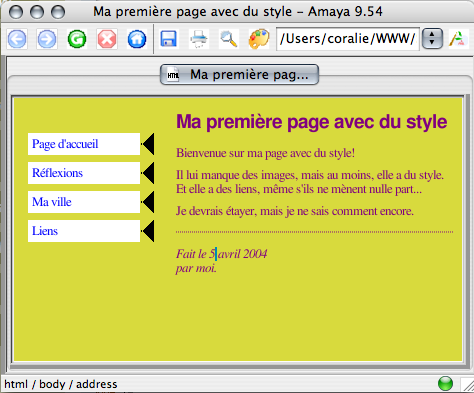
\includegraphics{voronin/img/capture5.png}
		\caption{Le texte principal a été déplacé à droite et la liste de liens est maintenant à sa gauche au lieu d'être au-dessus. }
		\label{fig:screen6}	
	\end{center}
\end{figure}
L'étape suivante est d'enregistrer les deux fichiers mapage.html et monstyle.css sur votre site Web. (Probablement après les avoir modifié un peu au préalable…) Mais cela dépend entièment de votre fournisseur d'accès Internet. 



\end{document}
